\documentclass{article}
\usepackage{geometry}
\geometry{margin=1in}
\usepackage{graphicx}
\usepackage{booktabs}
\usepackage{multirow}
\usepackage{float}
\usepackage{hyperref}
\usepackage{xcolor}
\usepackage{colortbl}
\definecolor{lightgray}{rgb}{0.95,0.95,0.95}
\definecolor{blue}{rgb}{0.0,0.0,0.8}
\definecolor{darkblue}{rgb}{0.0,0.0,0.5}
\title{\textcolor{blue}{Gunshot Detection Report}}
\author{Gunshot Detection System}
\date{\today}
\begin{document}
\maketitle

\section*{\textcolor{darkblue}{Audio File Information}}
\begin{table}[h]
\centering
\begin{tabular}{ll}
\toprule
\textbf{Parameter} & \textbf{Value} \\
\midrule
Filename & temp_clip.wav \\
Duration & 1.00 seconds \\
Sample Rate & 44100 Hz \\
\bottomrule
\end{tabular}
\end{table}

\section*{\textcolor{darkblue}{Spectrogram Analysis}}
\begin{figure}[h]
\centering
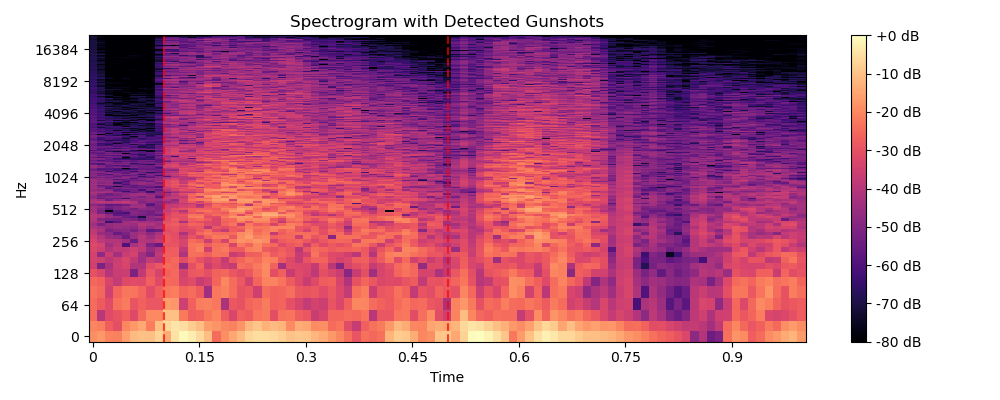
\includegraphics[width=\textwidth]{spectrogram_20250428_233129.png}
\caption{Spectrogram showing detected gunshots (marked in red)}
\end{figure}

\section*{\textcolor{darkblue}{Detected Gunshots}}
\begin{table}[h]
\centering
\begin{tabular}{cccc}
\toprule
\textbf{Timestamp (s)} & \textbf{Type} & \textbf{Caliber} & \textbf{Confidence (\%)} \\
\midrule
0.10 & Smith & Wesson & .38 cal & 95.0 \\
\midrule
0.50 & Smith & Wesson & .38 cal & 95.0 \\
\midrule
\bottomrule
\end{tabular}
\end{table}

\section*{\textcolor{darkblue}{Firearm Analysis}}
\begin{figure}[h]
\centering
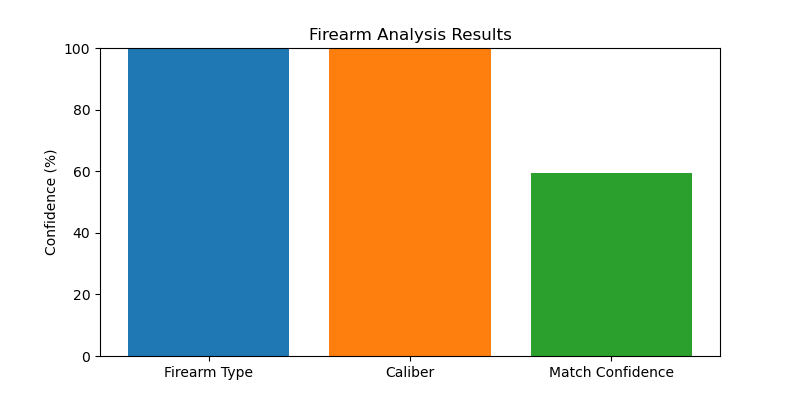
\includegraphics[width=0.8\textwidth]{firearm_analysis_20250428_233129.png}
\caption{Firearm analysis results}
\end{figure}
\begin{table}[h]
\centering
\begin{tabular}{ll}
\toprule
\textbf{Parameter} & \textbf{Value} \\
\midrule
Firearm Type & Glock 17 \\
Caliber & .38 cal \\
Match Confidence & 59.5\% \\
\bottomrule
\end{tabular}
\end{table}

\section*{\textcolor{darkblue}{Summary}}
This report contains the results of the comprehensive gunshot detection and analysis performed on the audio file. The analysis includes detection of gunshot events, their timestamps, and classification of the firearm type. The confidence levels are provided for each detection and classification.

\end{document}
